\documentclass[11pt]{article}
\usepackage[margin=1in]{geometry}
\usepackage[T1]{fontenc}
\usepackage{lmodern}
\usepackage{amsmath,amssymb}
\usepackage{graphicx}
\usepackage{booktabs}
\usepackage{caption}
\usepackage{microtype}
\usepackage[hidelinks]{hyperref}
\captionsetup{font=small,labelfont=bf,width=0.95\textwidth}
\graphicspath{{../figs/}}
% let text share a page with a tall figure instead of forcing float-only pages
\renewcommand{\topfraction}{0.95}
\renewcommand{\bottomfraction}{0.6}
\renewcommand{\textfraction}{0.05}
\renewcommand{\floatpagefraction}{0.85}

\newcommand{\eps}{\varepsilon}
\newcommand{\sci}[2]{$#1\times10^{#2}$}
\newcommand{\code}[1]{\texttt{#1}}

\title{Computational Physics, Homework 2:\\
Overrelaxation, Wien's displacement constant,
and gradient-descent fitting of the stellar mass function}
\author{Xuanzhe Xia \\ \texttt{xx2720@nyu.edu} \\[4pt]
\small Code: \url{https://github.com/hz-xiaxz/compphys-hw2}}
\date{October 5, 2026}

\begin{document}
\maketitle

\section*{Summary}

This assignment has three parts. In the first (Newman, Exercise~6.11) I solved
the nonlinear equation $x = 1-e^{-2x}$ to an accuracy of $10^{-6}$ by relaxation
and by overrelaxation. Linearizing the iteration about the solution gives an
error estimate that works for both methods and a prediction for the best
overrelaxation parameter, $\omega_{\mathrm{opt}} = f'(x^*)/[1-f'(x^*)] = 0.685$.
Plain relaxation needs 14 iterations; overrelaxation with $\omega$ near
$\omega_{\mathrm{opt}}$ needs 3--4, a reduction of more than a factor of three.
The same formula shows that a negative $\omega$ is the right choice whenever
$f'(x^*)<0$, and for $x=\cos x$ it cuts the iteration count from 32 to~3.

In the second part (Newman, Exercise~6.13) I showed that the peak of Planck's
law satisfies $5e^{-x}+x-5=0$ with $x = hc/\lambda k_BT$, and solved it by
binary search to an accuracy of $10^{-6}$ in 24 bisection steps:
$x = 4.965114$. This gives Wien's displacement constant
$b = hc/k_Bx = 2.897772\times10^{-3}\ \mathrm{m\,K}$. For a solar spectrum peaking
at $502\ \mathrm{nm}$, it gives a surface temperature of $5772\ \mathrm{K}$.

In the third part I wrote a multidimensional gradient-descent minimizer that uses
only function values (central-difference gradients), verified it on
$f(x,y) = (x-2)^2+(y-2)^2$, and used it to fit a Schechter function to the COSMOS
galaxy stellar mass function by minimizing $\chi^2$. Six starting points spread
over parameter space all converge to the same minimum, $\chi^2 = 2.91$ for 9
degrees of freedom, with $\log_{10}\phi^* = -2.568\pm0.064$,
$\log_{10}M^* = 10.976\pm0.044$ and $\alpha = -1.009\pm0.063$; the end points
agree to $\sim10^{-6}$, far below the statistical errors.

\section*{Methods}

\subsection*{Problem 1: relaxation and overrelaxation}

The relaxation method solves $x = f(x)$ by iterating $x' = f(x)$. Overrelaxation
pushes each step further by a factor $1+\omega$,
\[
x' = x + (1+\omega)\,[f(x)-x] = (1+\omega)f(x) - \omega x ,
\]
and reduces to relaxation for $\omega=0$.

\paragraph{(a) Error estimate.}
Write the current estimate as $x = x^*-\eps$, where $x^*$ is the exact solution,
and the next one as $x' = x^*-\eps'$. Expanding $f$ about $x^*$ and using
$f(x^*) = x^*$,
\[
x' = (1+\omega)\big[x^* - \eps f'(x^*) + O(\eps^2)\big] - \omega(x^*-\eps)
   = x^* - \big[(1+\omega)f'(x^*)-\omega\big]\eps ,
\]
so to first order $\eps' = g\,\eps$ with $g \equiv (1+\omega)f'(x^*)-\omega$.
Since $x^* = x+\eps = x'+\eps'$, we have $x'-x = \eps-\eps' = \eps'(1/g - 1)$, and
therefore
\[
\eps' \simeq \frac{x-x'}{1-1/\big[(1+\omega)f'(x^*)-\omega\big]} .
\]
The relation $\eps' = g\,\eps$ is the overrelaxation equivalent of Newman's
Eq.~(6.81), and the error formula is the equivalent of Eq.~(6.83); both reduce
to the relaxation results for $\omega=0$. The iteration
converges if $|g|<1$, linearly with ratio $g$, and is fastest when $g = 0$, i.e.\
for
\[
\omega_{\mathrm{opt}} = \frac{f'(x^*)}{1-f'(x^*)} .
\]

\paragraph{(b), (c) Implementation.}
For $f(x) = 1-e^{-cx}$ with $c=2$ I have $f'(x) = ce^{-cx}$. Since $x^*$ is not
known during the iteration, $f'(x^*)$ in the error formula is replaced by $f'$ at
the newest iterate, as in the book's form of the formula, and the iteration stops when $|\eps'|<10^{-6}$. Every run
starts from $x_0=1$. To check the stopping criterion I also computed $x^*$ to
machine precision with Brent's method (\code{scipy.optimize.brentq}) and
recorded the true error $|x_n-x^*|$ at each step. I scanned $\omega$ from $-0.9$
to $2.3$ in steps of $0.01$.

\paragraph{(d) Negative $\omega$.}
To test the prediction that $\omega<0$ helps when $f'(x^*)<0$, the same code was
run on $x = \cos x$, for which $f'(x^*) = -\sin x^* = -0.674$.

\subsection*{Problem 2: Wien's displacement constant}

\paragraph{(a) The peak of Planck's law.}
Write $I(\lambda) = 2\pi hc^2\lambda^{-5}/(e^{u}-1)$ with $u = hc/\lambda k_BT$,
so that $du/d\lambda = -u/\lambda$. Then
\[
\frac{dI}{d\lambda}
= 2\pi hc^2\left[\frac{-5\lambda^{-6}}{e^{u}-1}
  - \frac{\lambda^{-5}e^{u}}{(e^{u}-1)^2}\,\frac{du}{d\lambda}\right]
= \frac{2\pi hc^2\lambda^{-6}}{(e^{u}-1)^2}\Big[u\,e^{u} - 5\big(e^{u}-1\big)\Big].
\]
The prefactor never vanishes for finite $\lambda$, so $dI/d\lambda = 0$ requires
$ue^{u} = 5(e^{u}-1)$. Multiplying by $e^{-u}$ gives
\[
5e^{-hc/\lambda k_BT} + \frac{hc}{\lambda k_BT} - 5 = 0 .
\]
With $x = hc/\lambda k_BT$ this is $5e^{-x}+x-5=0$, which contains no physical
constants. Its root $x$ is therefore a pure number, and the peak wavelength is
\[
\lambda = \frac{hc}{k_B x}\,\frac{1}{T} = \frac{b}{T},\qquad
b = \frac{hc}{k_B x} .
\]
The equation also has the root $x=0$ ($\lambda\to\infty$), which is the limit
$I\to0$, not the maximum. For $0<x<x^*$ the bracket $ue^u-5(e^u-1)$ is negative,
so $dI/d\lambda<0$; for $x>x^*$ it is positive. The nonzero root is therefore a
maximum of $I(\lambda)$.

\paragraph{(b) Binary search.}
The function $g(x) = 5e^{-x}+x-5$ has $g(1) = 5/e-4 = -2.16$ and
$g(10) = +5.0002$, so $[1,10]$ brackets the nonzero root and excludes $x=0$.
At each step the bracket is halved and the half in which $g$ changes sign is
kept. The search stops when the bracket is narrower than $\eps = 10^{-6}$, and
the midpoint is returned, so the error is at most $\eps/2$. The number of steps
is fixed in advance at $\lceil\log_2[(10-1)/10^{-6}]\rceil = 24$. I used the
exact SI values $h = 6.62607015\times10^{-34}\ \mathrm{J\,s}$,
$c = 299\,792\,458\ \mathrm{m/s}$ and $k_B = 1.380649\times10^{-23}\ \mathrm{J/K}$.
To check the result, I also found the root to machine precision with Brent's method.


\subsection*{Problem 3: gradient descent and the Schechter fit}

\paragraph{The minimizer.}
Gradient descent steps downhill, $\mathbf{x}_{i+1} = \mathbf{x}_i -
\gamma\,\nabla f(\mathbf{x}_i)$. The gradient is never supplied analytically; each
component is a central difference,
\[
\frac{\partial f}{\partial x_k} \simeq
\frac{f(\mathbf{x}+h\hat{\mathbf{e}}_k) - f(\mathbf{x}-h\hat{\mathbf{e}}_k)}{2h},
\qquad h = 10^{-6},
\]
with truncation error $O(h^2)\sim10^{-12}$ and round-off error
$\sim\eps_m f/h \sim 10^{-10}f$ in double precision. The code supports a fixed
step $\gamma$ and an adaptive one: after each step that lowers $f$ the step is
multiplied by $1.2$, and a step that would raise $f$ is rejected and retried
with $\gamma$ halved. Optionally a single step is also capped at a maximum length.
The iteration stops when $|\nabla f|<10^{-8}$ or a step lowers $f$ by less
than $10^{-12}$ of its value.

\paragraph{Test.}
For $f(x,y) = (x-2)^2+(y-2)^2$ the exact gradient is $2(\mathbf{x}-\mathbf{x}^*)$,
so a fixed step gives $\mathbf{x}_{i+1}-\mathbf{x}^* = (1-2\gamma)(\mathbf{x}_i -
\mathbf{x}^*)$. With $\gamma=0.1$ the distance to the minimum should shrink by
exactly $0.8$ per step and $f$ by $0.64$. I ran the code with fixed $\gamma=0.1$
from four starting points.

\paragraph{The fit.}
The data file gives, for 12 bins of $\log_{10}M_{\mathrm{gal}}$ from 9.6 to 11.8,
the number density $n_i$ per dex per $(\mathrm{Mpc}/h)^3$ and its error
$\sigma_i$. The model is
\[
n(M) = \phi^*\left(\frac{M}{M^*}\right)^{\alpha+1}
\exp\!\left(-\frac{M}{M^*}\right)\ln 10 ,
\]
and the function minimized is
$\chi^2 = \sum_i [n(M_i)-n_i]^2/\sigma_i^2$. The choice of variables matters for
gradient descent, because the method only converges quickly when $\chi^2$ has
similar curvature in all directions. I fit
$\mathbf{p} = (\log_{10}\phi^*,\ \log_{10}M^*,\ \alpha)$, in which all three
parameters are of order unity and the eigenvalues of the Hessian of $\chi^2$ at
the minimum are $212$, $4690$ and $10\,908$ (condition number 51). In linear
$\phi^*$ the condition number is $\sim10^{6}$, and plain gradient descent would
crawl along the shallow direction.

The fit uses the adaptive step, starting at $\gamma=10^{-6}$, with each step
capped at a length of 0.2. Far from the minimum $\chi^2$ can be $10^{8}$ and its
gradient enormous, so without the cap a single step can throw the walker onto a
plateau where the model is essentially zero and the gradient vanishes. That
happened from one of the starting points before I added the cap. To test
robustness I started from six points spread over
$-4\le\log_{10}\phi^*\le-1.5$, $10\le\log_{10}M^*\le11.8$ and
$-1.8\le\alpha\le0$ (Table~\ref{tab:p3}). For comparison I also ran one fit with
a fixed step $\gamma = 1/\lambda_{\max}$, half the stability limit
$2/\lambda_{\max}$ set by the largest Hessian eigenvalue. Parameter
uncertainties come from the curvature at the minimum,
$\mathrm{Cov}(\mathbf{p}) = 2\,\mathbf{H}^{-1}$ with $\mathbf{H}$ the Hessian of
$\chi^2$ computed by second-order central differences. The result was
cross-checked against \code{scipy.optimize.least\_squares}.

\section*{Results}

\subsection*{Problem 1: overrelaxation}

\begin{figure}[htbp]
\centering
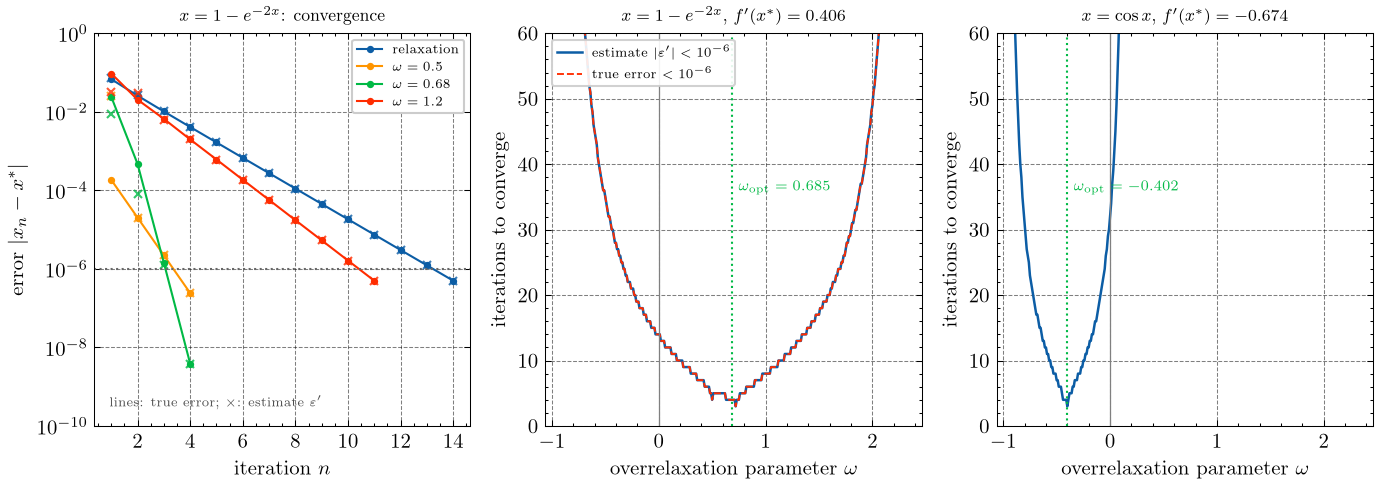
\includegraphics[width=\textwidth]{problem1_relaxation.png}
\caption{Left: true error $|x_n-x^*|$ (lines) and the estimate $\eps'$ of
part~(a) (crosses) for $x=1-e^{-2x}$ with ordinary relaxation and three values
of $\omega$; the dotted line is the target accuracy $10^{-6}$. Middle: number of
iterations needed to reach $10^{-6}$ as a function of $\omega$, using the
estimate as the stopping criterion (solid) and using the true error (dashed);
the dotted vertical line is the predicted $\omega_{\mathrm{opt}}=0.685$. Right:
the same scan for $x=\cos x$, where $f'(x^*)<0$ and the optimum lies at
$\omega_{\mathrm{opt}} = -0.402$.}
\label{fig:p1}
\end{figure}

The solution of $x = 1-e^{-2x}$ is $x^* = 0.796812$, where
$f'(x^*) = 2(1-x^*) = 0.406$.

\paragraph{(b) Relaxation.}
Ordinary relaxation from $x_0=1$ converges to $x = 0.796813$ in 14 iterations;
the true error at that point is \sci{5.0}{-7}. The left panel of
Fig.~\ref{fig:p1} shows the error shrinking by a constant factor
$f'(x^*)\approx0.41$ per step, as expected for linear convergence.

\paragraph{(c) Overrelaxation.}
Table~\ref{tab:p1} lists the iteration counts for several values of $\omega$.
Overrelaxation with $\omega = 0.5$--$0.7$ needs only 4--5 iterations, and the
fastest value in the scan, $\omega=0.72$, needs 3. This is better than the
factor-of-two reduction the exercise asks for. The minimum of the scan in the
middle panel of Fig.~\ref{fig:p1} sits at the predicted
$\omega_{\mathrm{opt}} = 0.685$, where $g=0$ and the linear error term vanishes.
At $\omega = 0.68$, $g = 0.003$, so after the first two steps the error falls by
a factor of $\sim370$ per step, from \sci{4.7}{-4} to \sci{3.9}{-9} in two steps
(left panel). Exactly at $\omega_{\mathrm{opt}}$ the linear term vanishes and
the convergence becomes quadratic. Too large
an $\omega$ overshoots: at $\omega=1.5$, $g = -0.48$, the iterates oscillate
about $x^*$ and the method is slower than plain relaxation, and for
$\omega\gtrsim2.37$ ($|g|>1$) it diverges. The crosses in the left panel lie
on the true errors, and the two scan curves in the middle panel are identical
at every $\omega$, so the error estimate of part~(a) is a reliable stopping criterion.
Every run that stopped on $|\eps'|<10^{-6}$ was within $10^{-6}$ of $x^*$.

\begin{table}[htbp]
\centering
\caption{Iterations needed to reach an estimated accuracy of $10^{-6}$ for
$x=1-e^{-2x}$, starting from $x_0=1$, and the true error of the final iterate.}
\label{tab:p1}
\begin{tabular}{cccc}
\toprule
$\omega$ & $g=(1+\omega)f'(x^*)-\omega$ & iterations & true error\\
\midrule
0 (relaxation) & $+0.41$ & 14 & \sci{5.0}{-7}\\
0.25 & $+0.26$ & 9 & \sci{6.1}{-7}\\
0.50 & $+0.11$ & 4 & \sci{2.4}{-7}\\
0.60 & $+0.05$ & 5 & \sci{1.0}{-7}\\
0.70 & $-0.01$ & 4 & \sci{2.2}{-8}\\
0.72 & $-0.02$ & 3 & \sci{3.9}{-8}\\
0.80 & $-0.07$ & 5 & \sci{5.0}{-7}\\
1.00 & $-0.19$ & 8 & \sci{3.9}{-7}\\
1.50 & $-0.48$ & 17 & \sci{8.9}{-7}\\
\bottomrule
\end{tabular}
\end{table}

\paragraph{(d) When does $\omega<0$ help?}
The best parameter $\omega_{\mathrm{opt}} = f'(x^*)/[1-f'(x^*)]$ is negative
whenever $f'(x^*)<0$. In that case relaxation already overshoots: the iterates
land alternately on either side of $x^*$, and the error changes sign at each
step with ratio $f'(x^*)$. Overrelaxing ($\omega>0$) makes the overshoot worse,
while $\omega<0$ damps each step (underrelaxation). For $x=\cos x$, with
$f'(x^*) = -0.674$, plain relaxation needs 32 iterations, $\omega = -0.2$ needs
12, and $\omega=-0.40\approx\omega_{\mathrm{opt}}$ needs only 3 (right panel of
Fig.~\ref{fig:p1}). A positive $\omega$ is harmful here: already at
$\omega=0.2$, $g=-1.008$ and the iteration diverges. Negative $\omega$ also helps
when $f'(x^*)>1$, where ordinary relaxation does not converge at all. Choosing
$\omega<-1$ then reverses the direction of the step and gives $|g|<1$. For
example, $\omega=-2$ makes the unstable root $x^*=0$ of $x=1-e^{-2x}$, where
$f'=2$, converge immediately.

\subsection*{Problem 2: Wien's displacement constant}

\begin{figure}[htbp]
\centering
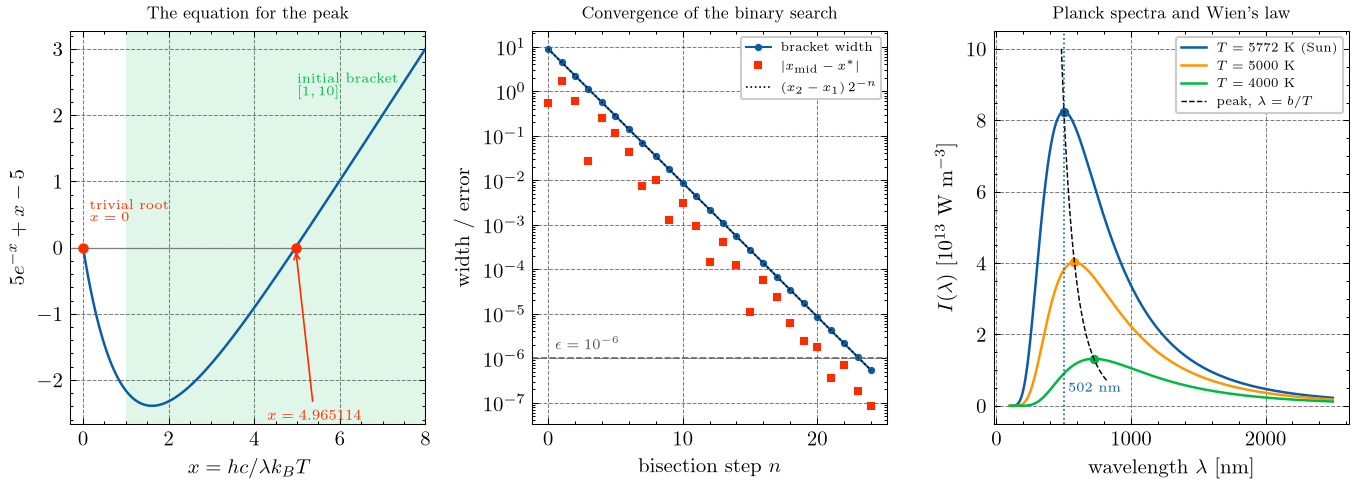
\includegraphics[width=\textwidth]{problem2_wien.png}
\caption{Left: $g(x) = 5e^{-x}+x-5$ with its trivial root $x=0$ and the
physical root $x=4.965114$; the shaded region is the initial bracket.
Middle: bracket width (blue), true error of the midpoint (red squares) and
$(x_2-x_1)2^{-n}$ (dotted) against bisection step; the dashed line is the
target accuracy $\eps=10^{-6}$. Right: Planck spectra $I(\lambda)$ for the Sun's
temperature found here and two cooler bodies. The points mark $\lambda=b/T$
from the computed $b$, and the dashed curve traces the peak as $T$ varies.}
\label{fig:p2}
\end{figure}

\paragraph{(b) Root and displacement constant.}
The binary search on $[1,10]$ takes 24 steps, as predicted, and returns
\[
x = 4.965114\quad(\text{final bracket width } 5.4\times10^{-7},\
\text{true error } 8.5\times10^{-8}).
\]
The bracket halves exactly at every step (middle panel of Fig.~\ref{fig:p2}).
The true error of the midpoint is always below the bracket width but does not
decrease monotonically, because the root can lie anywhere inside the bracket.
The displacement constant is
\[
b = \frac{hc}{k_Bx} = 2.897772\times10^{-3}\ \mathrm{m\,K},
\]
with an uncertainty from the bisection of $b\,\delta x/x\approx3\times10^{-10}\
\mathrm{m\,K}$ (one part in $10^{7}$). This agrees with the value from the
machine-precision root, $2.897771955\times10^{-3}\ \mathrm{m\,K}$, and with the
CODATA value of Wien's constant.

\paragraph{(c) The temperature of the Sun.}
With the peak of the solar spectrum at $\lambda = 502\ \mathrm{nm}$,
\[
T_\odot = \frac{b}{\lambda} = \frac{2.897772\times10^{-3}\ \mathrm{m\,K}}{502\times10^{-9}\ \mathrm{m}}
\approx 5772\ \mathrm{K}.
\]
This matches the Sun's effective temperature of about $5772\ \mathrm{K}$. The
precision is limited by the quoted wavelength, not by $b$: an uncertainty of
$1\ \mathrm{nm}$ in $\lambda$ changes $T_\odot$ by about $11\ \mathrm{K}$. In
addition, the real solar spectrum is only approximately a black body. The right
panel of Fig.~\ref{fig:p2} shows the Planck curve at this temperature peaking at
$502\ \mathrm{nm}$, and the peak shifting to longer wavelength as $T$ drops.


\subsection*{Problem 3: gradient descent and the Schechter fit}

\begin{figure}[htbp]
\centering
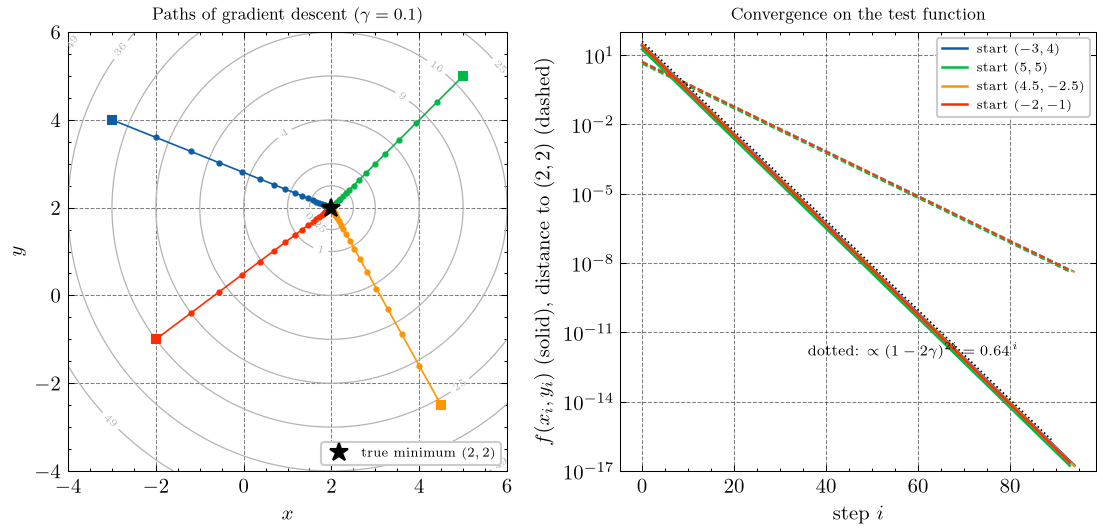
\includegraphics[width=0.95\textwidth]{problem3_test.png}
\caption{Test of the gradient-descent code on $f(x,y)=(x-2)^2+(y-2)^2$ with a
fixed step $\gamma=0.1$ and numerical gradients. Left: paths from four starting
points (squares) over contours of $f$. Right: $f$ (solid) and the distance to
$(2,2)$ (dashed) as a function of step. The dotted line is the exact rate
$0.64^{\,i}$ for $f$.}
\label{fig:p3test}
\end{figure}

\paragraph{Test function.}
From all four starting points the code walks straight to $(2,2)$
(Fig.~\ref{fig:p3test}) and stops after 93--94 steps at
$(2.00000000, 2.00000000)$ with $f\approx2\times10^{-17}$. The function value
falls by exactly the predicted factor $(1-2\gamma)^2 = 0.64$ per step over 17
decades, so the numerical gradient is accurate enough not to affect the
convergence.

\begin{figure}[htbp]
\centering
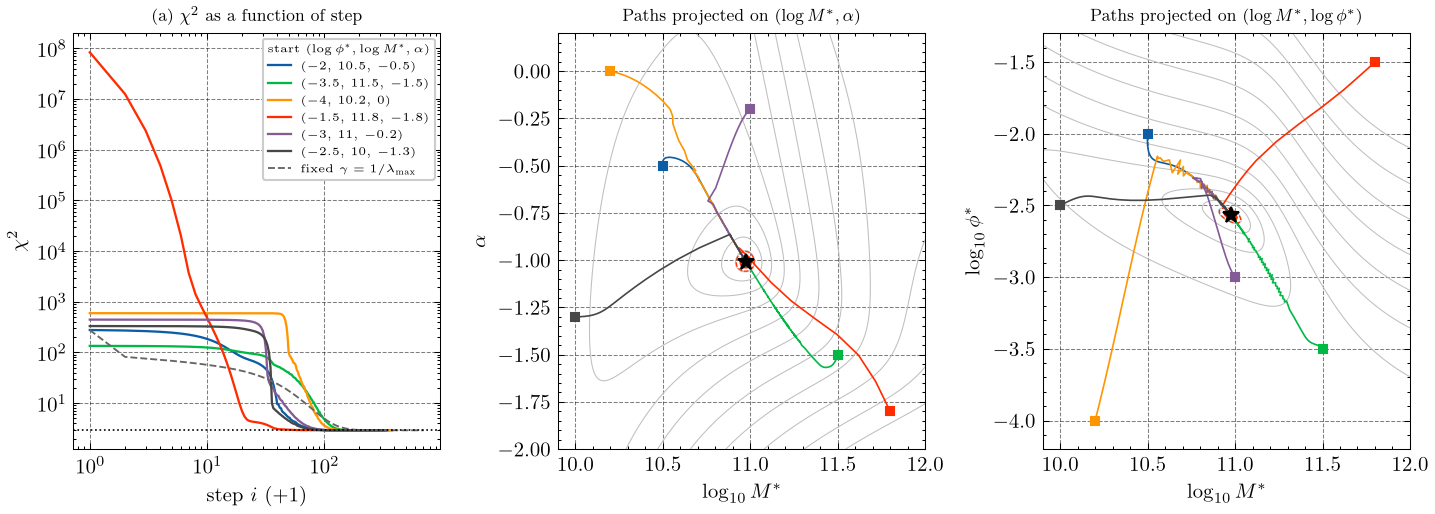
\includegraphics[width=\textwidth]{problem3_chi2.png}
\caption{(a) $\chi^2$ of the Schechter fit as a function of gradient-descent
step from six starting points (legend), on logarithmic axes; the dotted line is
the minimum $\chi^2 = 2.908$. The dashed grey curve is a run with a fixed step
$\gamma = 1/\lambda_{\max}$. Middle and right: the same paths projected onto
two parameter planes, over contours of $\log_{10}\chi^2$ with the third
parameter held at its best-fit value. The small red ellipses around the star
are $\Delta\chi^2 = 2.30$ and $6.18$ (68\% and 95\% for two parameters).}
\label{fig:p3chi2}
\end{figure}

\begin{figure}[htbp]
\centering
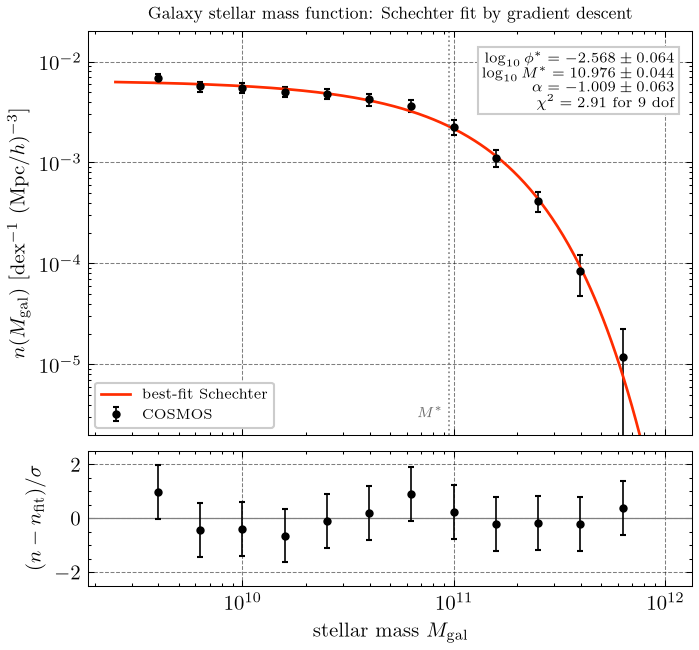
\includegraphics[width=0.62\textwidth]{problem3_fit.png}
\caption{(b) The COSMOS stellar mass function (points with $1\sigma$ errors)
and the best-fit Schechter function found by gradient descent (red), on
logarithmic axes. The dotted vertical line marks $M^*$. The lower panel shows
the residuals in units of $\sigma$.}
\label{fig:p3fit}
\end{figure}

\paragraph{$\chi^2$ versus step.}
Figure~\ref{fig:p3chi2}(a) shows $\chi^2$ along each path. The starting values
range from $\chi^2\approx130$ to $8\times10^{7}$. Every run goes through the
same stages: a slow phase while the steps are still tiny (the adaptive $\gamma$
starts at $10^{-6}$), a rapid drop of one to seven decades once $\gamma$ has
grown, and a slow final approach along the shallowest direction of the
$\chi^2$ valley, which in the projections of Fig.~\ref{fig:p3chi2} is a
diagonal valley. This valley reflects the strong correlations between the
parameters (correlation coefficients $-0.89$ between $\log\phi^*$ and
$\log M^*$, $+0.94$ between $\log\phi^*$ and $\alpha$): a higher $M^*$ can be
traded against a lower amplitude and a steeper slope. The runs converge in
287--381 steps. The fixed-step run with $\gamma=1/\lambda_{\max}$ also reaches
the minimum but needs 711 steps, because a step small enough to be stable along
the steepest direction is too small along the shallowest one.

\paragraph{Robustness.}
Table~\ref{tab:p3} lists the end point of each run. All six give
$\chi^2 = 2.908056$ and the same parameters to within
\sci{1.6}{-6} in every coordinate, more than $10^{4}$ times smaller than the
statistical errors. The result is therefore independent of the starting
point, and \code{scipy.optimize.least\_squares} finds the same minimum.

\begin{table}[htbp]
\centering
\caption{End points of gradient descent for six starting points
$(\log_{10}\phi^*,\log_{10}M^*,\alpha)$.}
\label{tab:p3}
\begin{tabular}{lccccc}
\toprule
start & steps & $\chi^2$ & $\log_{10}\phi^*$ & $\log_{10}M^*$ & $\alpha$\\
\midrule
$(-2.0, 10.5, -0.5)$ & 343 & 2.908056 & $-2.56822$ & 10.97623 & $-1.00939$\\
$(-3.5, 11.5, -1.5)$ & 381 & 2.908056 & $-2.56822$ & 10.97623 & $-1.00939$\\
$(-4.0, 10.2, \phantom{-}0.0)$ & 373 & 2.908056 & $-2.56821$ & 10.97623 & $-1.00939$\\
$(-1.5, 11.8, -1.8)$ & 287 & 2.908056 & $-2.56821$ & 10.97623 & $-1.00939$\\
$(-3.0, 11.0, -0.2)$ & 346 & 2.908056 & $-2.56822$ & 10.97623 & $-1.00939$\\
$(-2.5, 10.0, -1.3)$ & 327 & 2.908056 & $-2.56821$ & 10.97623 & $-1.00939$\\
\bottomrule
\end{tabular}
\end{table}

\paragraph{Best fit.}
The best-fit Schechter parameters, with $1\sigma$ errors from the curvature of
$\chi^2$, are
\begin{align*}
\log_{10}\phi^* &= -2.568\pm0.064 &
&\big(\phi^* = (2.70\pm0.40)\times10^{-3}\ (\mathrm{Mpc}/h)^{-3}\big),\\
\log_{10}M^* &= 10.976\pm0.044, & \alpha &= -1.009\pm0.063 .
\end{align*}
Figure~\ref{fig:p3fit} compares the fit with the data. The model follows the
nearly flat low-mass end, where $\alpha\approx-1$ means equal numbers of galaxies
per logarithmic mass interval, and the exponential cut-off above
$M^*\approx10^{11}$, where the density drops by more than two decades between
$10^{11}$ and $10^{11.8}$. All residuals are within $1\sigma$ (the largest is $+0.99\sigma$, in the
lowest-mass bin). The minimum $\chi^2 = 2.91$ for $12-3 = 9$ degrees of freedom
(reduced $\chi^2 = 0.32$; a value this low or lower has a probability of about
3\% for a correct model with independent Gaussian errors) suggests that the
quoted errors are conservative or correlated between mass bins, as they would
be if they include cosmic variance, which a diagonal $\chi^2$ ignores. The
Schechter form describes the data well. The parameter errors above assume
independent errors and should be read as rough estimates.

\section*{Code}

All code, the data, the figures and the numerical outputs are in the public
GitHub repository \code{hz-xiaxz/compphys-hw2}:
\begin{center}
\url{https://github.com/hz-xiaxz/compphys-hw2}
\end{center}
The scripts are plain Python (NumPy, SciPy, Matplotlib, SciencePlots) managed
with \code{uv}:
\begin{itemize}
\item \code{problem1.py}: relaxation and overrelaxation with the error estimate
of part~(a), the $\omega$ scans, and \path{figs/problem1_relaxation.png}.
\item \code{problem2.py}: the binary search for $5e^{-x}+x-5=0$, Wien's
constant and the solar temperature, and \path{figs/problem2_wien.png}.
\item \code{problem3.py}: the gradient-descent minimizer with numerical
gradients, the test on $(x-2)^2+(y-2)^2$, the Schechter fit from six starting
points, the Hessian error estimate, and \path{figs/problem3_test.png},
\path{figs/problem3_chi2.png} and \path{figs/problem3_fit.png}.
\item \code{plotstyle.py}: shared figure style. \code{results/} holds the
printed output of each script, and \code{writeup/} holds the source of this
document.
\end{itemize}
Running \code{uv sync} followed by \code{uv run python problemN.py} reproduces
every figure and number quoted here.

\end{document}
